%%\documentclass[a4paper,10pt]{jarticle}
%%\documentclass[]{jarticle}
%\documentclass[10pt]{jarticle}
%
%%\usepackage{graphicx}
%\usepackage[dvipdfmx]{graphicx}
%\usepackage{eclbkbox} %breakbox用
%\usepackage{listings,jlisting}
%
%%本文領域を広め(空白箇所マージン領域を小さめ)に設定
%\setlength{\textwidth}{179mm}
%\setlength{\textheight}{251mm}
%\setlength{\topmargin}{-2cm}
%\setlength{\oddsidemargin}{-1cm}
%\setlength{\evensidemargin}{-1cm}

%\documentclass[a4paper,10pt]{jarticle}
%\documentclass[]{jarticle}
\documentclass[10pt]{jarticle}

%\usepackage{graphicx}
\usepackage[dvipdfmx]{graphicx}
\usepackage{eclbkbox} %breakbox用
\usepackage{amsmath,amssymb}
\usepackage{verbatim}
\usepackage{moreverb}
\usepackage{ascmac,here,txfonts,txfonts}
\usepackage{listings,jlisting}
\usepackage{color}
\usepackage{fancybox}

%本文領域を広め(空白箇所マージン領域を小さめ)に設定
\lstset{
  breaklines = true,
  language=Python,
  basicstyle=\ttfamily\scriptsize,
  commentstyle={\itshape \color[cmyk]{1,0.4,1,0}},
  classoffset=1,
  keywordstyle={\bfseries \color[cmyk]{0,1,0,0}},
  stringstyle={\ttfamily \color[rgb]{0,0,1}},
  frame=tRBl,
  framesep=5pt,
  showstringspaces=false,
  numbers=left,
  stepnumber=1,
  numberstyle=\tiny,
  tabsize=2,
}

\setlength{\textwidth}{179mm}
\setlength{\textheight}{251mm}
\setlength{\topmargin}{-2cm}
\setlength{\oddsidemargin}{-1cm}
\setlength{\evensidemargin}{-1cm}


\begin{document}

\title{情報工学実験IIレポート(探索アルゴリズム2)}
\author{ 月曜班  グループ7} %
\date{実験実施日2014年12月22日}

\maketitle


\section*{グループメンバ}
\begin{itemize}
 \item 135711F:屋比久祐樹:Level1
 \item 135713B 天願寛之: 担当Level2.1
 \item 135717E 岡田和也: 担当Level3.1, 3.2
 \item 135761B 大城海斗: 担当Level2, 3.4
\end{itemize}

\section*{提出したレポート一式について}
レポート一式は
\verb|``naha:/home/home/teacher/tnal/jikken1-fri/e945734/''|
にアップロードした。
提出したファイルのディレクトリ構成は以下の通りである。\\
(補足:必ず下記のように整理しろという指定ではない。
自分たちでやりやすいようにLevel毎に整理しても構わない)
\begin{breakbox}
\begin{verbatim}
./src/      # 作成したプログラム一式
./report/   # レポート関係ファイル.図ファイルを含む.
\end{verbatim}
\end{breakbox}

\newpage

\section{Level1: 線形分離可能なOR問題への適用}
\subsection{OR$BLdBj$r3X=,$5$;$?:]$N8m:9<}B+EY9g$$$K$D$$$F(B}
\subsubsection{$B<B837k2L(B}
$B!!(B1000$B!A(B10000$B$N%7!<%ICM$rJQ$($k;v$K$h$j!"<}B+2s?t$,JQ2=$7(B10$B%Q%?!<%s$N8m:9$J$I$,?^(B1$B$GI=$;$k$3$H$G<B9T7k2L$,I=$l$?!#(B\\
$B!!$5$i$K!"(B10$B%Q%?!<%s$NJ?6Q7k2L$r?^(B2$B$H$7$F7k2L$,I=$l$?!#(B\\
\begin{table}[htb]
 \begin{center}
  \caption{OR$BLdBj$N3X=,$KMW$7$?2s?t(B}
  \label{table:level1}
  \begin{tabular}[htb]{r|l} \hline
   $B%7!<%ICM(B & $B<}B+$7$?2s?t(B \\ \hline \hline
   1000 & 96 \\ \hline
   2000 & 90 \\ \hline
   3000 & 111 \\ \hline
   4000 & 109 \\ \hline
   5000 & 93 \\ \hline
   6000 & 99 \\ \hline
   7000 & 100 \\ \hline
   8000 & 114 \\ \hline
   9000 & 113 \\ \hline
   10000 & 94 \\ \hline \hline
   10$B;n9T$NJ?6QCM(B & 101.9 \\ \hline
  \end{tabular}
 \end{center}
\end{table}

\begin{figure}[h]
 \begin{center}
  \includegraphics[width=10.0cm]{figs/1.eps}
  \caption{$B=E$_$r99?7$9$kMM;R(B}
  \label{fig:level1-1}
 \end{center}
\end{figure}

\begin{figure}[h]
 \begin{center}
  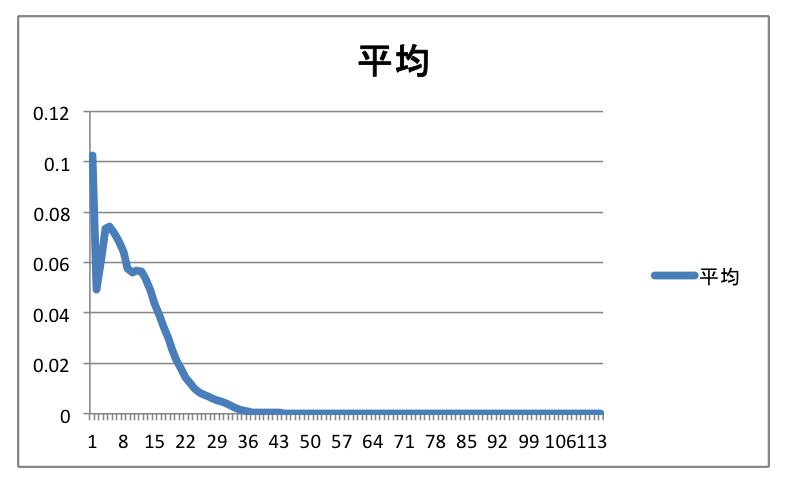
\includegraphics[width=10.0cm]{figs/2.eps}
  \caption{$B=E$_$r99?7$9$kMM;R!JJ?6QCM!K(B}
  \label{fig:level1-2}
 \end{center}
\end{figure}


\subsubsection{$B9M;!(B}
 $B>e5-$NFs$D$N?^$r8+$F(Bx$B<4$O<}B+2s?t$rI=$7!"(By$B<4$O8m:9$rI=$7$F$$$k!#?^#1$O(B10$B%Q%?!<%s$r$^$H$a<}B+2s?t$H8m:9$rI=$7$F$$$k!#?^#2$O(B10$B%Q%?!<%s$N%0%i%UJ?6Q$r$^$H$a$??^$G$"$k!#(B\\



 %課題説明
\subsection{OR$BLdBj$r3X=,$5$;$?:]$N8m:9<}B+EY9g$$$K$D$$$F(B}
\subsubsection{$B<B837k2L(B}
$B!!(B1000$B!A(B10000$B$N%7!<%ICM$rJQ$($k;v$K$h$j!"<}B+2s?t$,JQ2=$7(B10$B%Q%?!<%s$N8m:9$J$I$,?^(B1$B$GI=$;$k$3$H$G<B9T7k2L$,I=$l$?!#(B\\
$B!!$5$i$K!"(B10$B%Q%?!<%s$NJ?6Q7k2L$r?^(B2$B$H$7$F7k2L$,I=$l$?!#(B\\
\begin{table}[htb]
 \begin{center}
  \caption{OR$BLdBj$N3X=,$KMW$7$?2s?t(B}
  \label{table:level1}
  \begin{tabular}[htb]{r|l} \hline
   $B%7!<%ICM(B & $B<}B+$7$?2s?t(B \\ \hline \hline
   1000 & 96 \\ \hline
   2000 & 90 \\ \hline
   3000 & 111 \\ \hline
   4000 & 109 \\ \hline
   5000 & 93 \\ \hline
   6000 & 99 \\ \hline
   7000 & 100 \\ \hline
   8000 & 114 \\ \hline
   9000 & 113 \\ \hline
   10000 & 94 \\ \hline \hline
   10$B;n9T$NJ?6QCM(B & 101.9 \\ \hline
  \end{tabular}
 \end{center}
\end{table}

\begin{figure}[h]
 \begin{center}
  \includegraphics[width=10.0cm]{figs/1.eps}
  \caption{$B=E$_$r99?7$9$kMM;R(B}
  \label{fig:level1-1}
 \end{center}
\end{figure}

\begin{figure}[h]
 \begin{center}
  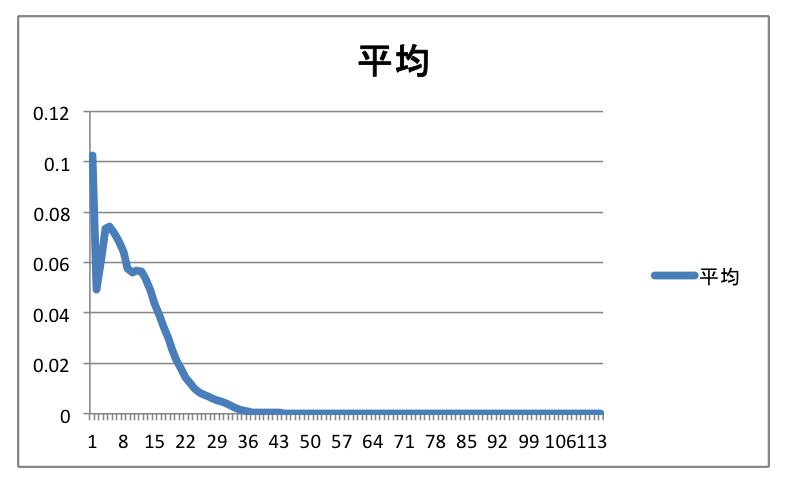
\includegraphics[width=10.0cm]{figs/2.eps}
  \caption{$B=E$_$r99?7$9$kMM;R!JJ?6QCM!K(B}
  \label{fig:level1-2}
 \end{center}
\end{figure}


\subsubsection{$B9M;!(B}
 $B>e5-$NFs$D$N?^$r8+$F(Bx$B<4$O<}B+2s?t$rI=$7!"(By$B<4$O8m:9$rI=$7$F$$$k!#?^#1$O(B10$B%Q%?!<%s$r$^$H$a<}B+2s?t$H8m:9$rI=$7$F$$$k!#?^#2$O(B10$B%Q%?!<%s$N%0%i%UJ?6Q$r$^$H$a$??^$G$"$k!#(B\\





\newpage

\section{Level2: 線形分離不可能なExOR問題への適用}
\subsection{階層型NNによる学習}
\subsubsection{最適なパラメータを探すためのアプローチ}
% 指定された条件下において学習が効率良く行われるパラメータの組み合わせを探
% すため、**して**することでパラメータを調整した。
% 
% (補足:全パターンを調べても良いし、いくつかのパターンを調べても良いが、
% どのような方法で調整したら良いかを考えよう)

$ETA,ALPHA,HIDDEN$を指定された範囲内でランダムな値に設定し,
プログラムを実行した.
パラメータの値の決定や,iteration数の平均値を求める処理は
次のシェルスクリプト(ソースコード\ref{level2})で行った.
ExOR問題は線形分離不可であるため,HIDDENの最小値を2としている.
最大値は特に指定されていないが,HIDDENを極端に大きくしすぎると
各パラメータの最適な組み合わせを見つけ出すのが困難になると考えたため,
最大値を16とした.


\lstinputlisting[caption=本levelで使用したシェルスクリプト,label=level2]{./level2figs/level2.sh}

このシェルスクリプトを数十回実行し,
iteration数の平均値が比較的小さい実行結果を10個分記録した.
その中で平均値が最小なものを選択し,グラフ化することにした.
%また出力結果の文字列を処理するため,
%bp\_mo\_exor.cの終了条件$FINISH$を出力するfprintf関数のstderrをstdoutへと変更を行った(ソースコード\ref{exor}).
%
%\lstinputlisting[caption=bp\_mo\_exor.cの変更点,label=exor]{./level2figs/exor.c}
%

\subsubsection{実行結果}

% (補足:シード値10パターンで試した際の収束に要した学習回数と、その平均回数が分かるように明示してください。)

表\ref{table:level2}にシード値10パターンで試した際の収束に要した学習回数と,その最小の平均回数を示す.

\begin{table}[htb]
 \begin{center}
  \begin{tabular}[htb]{|r|l|} \hline
   シード値 & 収束した回数 \\ \hline \hline
   1000     & 37\\ \hline
   2000     & 45\\ \hline
   3000     & 52\\ \hline
   4000     & 44\\ \hline
   5000     & 50\\ \hline
   6000     & 53\\ \hline
   7000     & 39\\ \hline
   8000     & 29\\ \hline
   9000     & 38\\ \hline
   10000    & 39 \\ \hline \hline
   10試行の平均値 & 42 \\ \hline
  \end{tabular}
  \caption{階層型NNによるExOR問題の学習に要した回数}
  \label{table:level2}
 \end{center}
\end{table}

各パラメータが$ETA=1.26, ALPHA=0.94, HIDDEN=16$の時,表\ref{table:level2}のような結果が得られた.
その時の学習曲線は図\ref{fig:averageultimate}のようになる.
図\ref{fig:averageultimate}はgnuplotを用いてseed値別にプロットしたグラフを元にsmooth uniqueオプションで平均化を行い,得られたものである.

\begin{figure}[h]
 \begin{center}
  \includegraphics[width=10.0cm]{./level2figs/averageultimate.eps}
  \caption{重みを更新する様子(平均値)}
  \label{fig:averageultimate}
 \end{center}
\end{figure}


\subsubsection{考察}
ここでは,各パラメータとiteration数の関係について考察する. \\
 下記に平均iteration数が比較的小さい実行結果とそのときのパラメータの値を示す.
\begin{itembox}[c]{平均iteration数が小さい実行結果}
    {\small
        \verbatimtabinput{./level2figs/suitables.txt}
    }
\end{itembox}
10回の実行結果における共通点は,いずれもALPHA値が1に近い値をとるという点だった. \\
 続いて,平均iteration数が大きい実行結果を示す.

\begin{itembox}[c]{平均iteration数が大きい実行結果}
    {\small
        \verbatimtabinput{./level2figs/unsuitables.txt}
    }
\end{itembox}

平均iteration数が小さいときのパラメータと平均iteration数が大きいときのそれとを比較すると,
HIDDENの値が小さいと平均iteration数が大きくなり,
反対に値が大きいと平均試行回数が小さくなるという結果になった.
また$ETA$に関しては,0を設定しない限りiteration数に大きな影響を
与えないことが伺える.
%また,$ETA$の値が0だと学習回数が100000を越える結果となった.
%これら実行結果より,$ETA,ALPHA,HIDDEN$は
これら実行結果より,最も効率良く学習が収束するパラメータの組み合わせは,表\ref{table:parameters}のようになる.

\begin{table}[htb]
 \begin{center}
  \begin{tabular}[htb]{|c|c|c|} \hline
   $ETA$ & $ALPHA$ & $HIDDEN$ \\ \hline \hline
   0以外の数値 & 1に近い値 & できるだけ大きい数値\\ \hline
  \end{tabular}
  \caption{最適なパラメータの組み合わせ}
  \label{table:parameters}
 \end{center}
\end{table}
 %共通部分の結果及び考察
\subsection{階層型NNによる学習}
\subsubsection{最適なパラメータを探すためのアプローチ}
% 指定された条件下において学習が効率良く行われるパラメータの組み合わせを探
% すため、**して**することでパラメータを調整した。
% 
% (補足:全パターンを調べても良いし、いくつかのパターンを調べても良いが、
% どのような方法で調整したら良いかを考えよう)

$ETA,ALPHA,HIDDEN$を指定された範囲内でランダムな値に設定し,
プログラムを実行した.
パラメータの値の決定や,iteration数の平均値を求める処理は
次のシェルスクリプト(ソースコード\ref{level2})で行った.
ExOR問題は線形分離不可であるため,HIDDENの最小値を2としている.
最大値は特に指定されていないが,HIDDENを極端に大きくしすぎると
各パラメータの最適な組み合わせを見つけ出すのが困難になると考えたため,
最大値を16とした.


\lstinputlisting[caption=本levelで使用したシェルスクリプト,label=level2]{./level2figs/level2.sh}

このシェルスクリプトを数十回実行し,
iteration数の平均値が比較的小さい実行結果を10個分記録した.
その中で平均値が最小なものを選択し,グラフ化することにした.
%また出力結果の文字列を処理するため,
%bp\_mo\_exor.cの終了条件$FINISH$を出力するfprintf関数のstderrをstdoutへと変更を行った(ソースコード\ref{exor}).
%
%\lstinputlisting[caption=bp\_mo\_exor.cの変更点,label=exor]{./level2figs/exor.c}
%

\subsubsection{実行結果}

% (補足:シード値10パターンで試した際の収束に要した学習回数と、その平均回数が分かるように明示してください。)

表\ref{table:level2}にシード値10パターンで試した際の収束に要した学習回数と,その最小の平均回数を示す.

\begin{table}[htb]
 \begin{center}
  \begin{tabular}[htb]{|r|l|} \hline
   シード値 & 収束した回数 \\ \hline \hline
   1000     & 37\\ \hline
   2000     & 45\\ \hline
   3000     & 52\\ \hline
   4000     & 44\\ \hline
   5000     & 50\\ \hline
   6000     & 53\\ \hline
   7000     & 39\\ \hline
   8000     & 29\\ \hline
   9000     & 38\\ \hline
   10000    & 39 \\ \hline \hline
   10試行の平均値 & 42 \\ \hline
  \end{tabular}
  \caption{階層型NNによるExOR問題の学習に要した回数}
  \label{table:level2}
 \end{center}
\end{table}

各パラメータが$ETA=1.26, ALPHA=0.94, HIDDEN=16$の時,表\ref{table:level2}のような結果が得られた.
その時の学習曲線は図\ref{fig:averageultimate}のようになる.
図\ref{fig:averageultimate}はgnuplotを用いてseed値別にプロットしたグラフを元にsmooth uniqueオプションで平均化を行い,得られたものである.

\begin{figure}[h]
 \begin{center}
  \includegraphics[width=10.0cm]{./level2figs/averageultimate.eps}
  \caption{重みを更新する様子(平均値)}
  \label{fig:averageultimate}
 \end{center}
\end{figure}


\subsubsection{考察}
ここでは,各パラメータとiteration数の関係について考察する. \\
 下記に平均iteration数が比較的小さい実行結果とそのときのパラメータの値を示す.
\begin{itembox}[c]{平均iteration数が小さい実行結果}
    {\small
        \verbatimtabinput{./level2figs/suitables.txt}
    }
\end{itembox}
10回の実行結果における共通点は,いずれもALPHA値が1に近い値をとるという点だった. \\
 続いて,平均iteration数が大きい実行結果を示す.

\begin{itembox}[c]{平均iteration数が大きい実行結果}
    {\small
        \verbatimtabinput{./level2figs/unsuitables.txt}
    }
\end{itembox}

平均iteration数が小さいときのパラメータと平均iteration数が大きいときのそれとを比較すると,
HIDDENの値が小さいと平均iteration数が大きくなり,
反対に値が大きいと平均試行回数が小さくなるという結果になった.
また$ETA$に関しては,0を設定しない限りiteration数に大きな影響を
与えないことが伺える.
%また,$ETA$の値が0だと学習回数が100000を越える結果となった.
%これら実行結果より,$ETA,ALPHA,HIDDEN$は
これら実行結果より,最も効率良く学習が収束するパラメータの組み合わせは,表\ref{table:parameters}のようになる.

\begin{table}[htb]
 \begin{center}
  \begin{tabular}[htb]{|c|c|c|} \hline
   $ETA$ & $ALPHA$ & $HIDDEN$ \\ \hline \hline
   0以外の数値 & 1に近い値 & できるだけ大きい数値\\ \hline
  \end{tabular}
  \caption{最適なパラメータの組み合わせ}
  \label{table:parameters}
 \end{center}
\end{table}


\newpage

\section{Level3: 応用事例:文字認識問題への適用}
\subsection{$B2]Bj@bL@(B}
$B3,AX7?(BNN$B$rJ8;zG'<1$KE,MQ$7!"9M;!$9$k!#(B
$BFC$K!"MQ0U$5$l$?65;U%G!<%?$HG'<1$N$7$d$9$5$K4X$9$k4X78@-$d!"(B
$B3X=,:GE,2=$N$?$a$N%Q%i%a!<%?$N%A%e!<%K%s%0$*$h$S!"(B
$B$h$j=@Fp@-$N9b$$G'<1J}K!$K4X$9$k8!F$$r9T$&!#(B

 %課題説明
\subsection{Level3.1: パラメータのチューニング}%
\subsubsection{最適なパラメータを探すためのアプローチ}
指定された条件下において学習が効率良く行われるパラメータの組み合わせを探
すため、
hiddenを10から100まで10づつ増やしていき,etaを0.01から1.98まで0.01づつ増
やし,alphaを0.1から1.0まで0.1づつ増やしていきその中から一番値が小さい物
を探した.その動作をスクリプトを書いて実行させた.
その後その値の近辺をスクリプトで探した.
\subsubsection{実行結果}
各パラメータがeta = 1.95, ALPHA = 0.62, HIDDEN 30の時,表5のよ
うな結果が得られたその時の学習曲線の平均はerrorを一回の学習ごとに足し,
それをまだ終了していないパターンの個数で割って出した.例えば61回目の学習
でシード値10000のパターンは収束しているので62回目の場合はerrorを足して9で
割ることで平均をだした.
\begin{table}[htb]
 \begin{center}
  \caption{階層型NNによる文字認識問題の学習に要した回数}
  \label{table:level3}
  \begin{tabular}[htb]{r|l} \hline
   シード値 & 収束した回数 \\ \hline \hline
   1000 & 105 \\ \hline
   2000 & 75 \\ \hline
   3000 & 62 \\ \hline
   4000 & 126 \\ \hline
   5000 & 74 \\ \hline
   6000 & 87 \\ \hline
   7000 & 85 \\ \hline
   8000 & 78 \\ \hline
   9000 & 122 \\ \hline
   10000 & 61 \\ \hline \hline
   10試行の平均値 & 87.5 \\ \hline
  \end{tabular}
 \end{center}
\end{table}

\begin{figure}[h]
 \begin{center}
  \includegraphics[width=10.0cm]{./figs/average.eps}
  \caption{重みを更新する様子(平均値)}
  \label{fig:level2}
 \end{center}
\end{figure}
\newpage



\subsection{Level3.2: $B%Q%i%a!<%?$H<}B+G=NO$N4XO"@-$K$D$$$F(B}
\subsubsection{$B4X78@-$r3NG'$9$k$?$a$N%"%W%m!<%A(B}
3$B$D$N%Q%i%a!<%?$,$I$N$h$&$J4X78$K$"$k$+$r8!>Z$9$k$?$a!"(B
$B%1!<%9(B1,2,,,$B$r@_Dj$7!"3X=,6J@~$+$i$=$N4X78@-$K$D$$$F9M;!$9$k!#(B

\subsubsection{$B7k2L(B}

\subsubsection{$B9M;!(B}


\subsection{Level3.3: 任意の評価用データを用いた評価}
\subsubsection{アプローチ}
学習時のデータ(教師データ)との違いが少ないほど認識率が高く、逆に教師データとの違いが多いほど認識率が低くなるとの仮定のもと、以下に示す評価用データを用意した。\\
今回は違いを分かり易くするため、0と1で表現された教師用データから、1の位置をズラす範囲とその数によって違いを作っている。つまり、より多くの1がより大きくズレていれば、より違いが多いということである。
\begin{figure}[htbp]
  \begin{center}
    \begin{tabular}{c}

      % 1
      \begin{minipage}{0.33\hsize}
        \begin{center}
          \includegraphics[clip, width=3.2cm]{./lebel3-3figs/eva1-3.pdf}
          \hspace{2.3cm} (1)違いが1番少ないデータ
        \end{center}
      \end{minipage}

      % 2
      \begin{minipage}{0.33\hsize}
        \begin{center}
          \includegraphics[clip, width=3.2cm]{./lebel3-3figs/eva1-4.pdf}
          \hspace{2.3cm} (2)違いが2番目に少ないデータ
        \end{center}
      \end{minipage}

      % 3
      \begin{minipage}{0.33\hsize}
        \begin{center}
          \includegraphics[clip, width=3.2cm]{./lebel3-3figs/eva1-5.pdf}
          \hspace{2.3cm} (3)違いが最も多いデータ
        \end{center}
      \end{minipage}

    \end{tabular}
    \caption{任意の評価用データ}
  \end{center}
\end{figure}

\subsubsection{結果}
最初に「1」という文字を学習させた。学習したことによる学習度合いを図6に示す。\\
\begin{figure}[htbp]
  \begin{center}
    \includegraphics[clip,width=5.5cm]{./lebel3-3figs/c.pdf}
    \caption{学習事例に対する学習度合いを確認}
  \end{center}
\end{figure}
\\用意した任意の評価用データに対する適応度合いを確認する。
\begin{figure}[htbp]
  \begin{center}
    \begin{tabular}{c}

      % 1
      \begin{minipage}{0.33\hsize}
        \begin{center}
          \includegraphics[clip, width=5.0cm]{./lebel3-3figs/e1.pdf}
          \hspace{2.3cm} (1)違いが1番少ないデータ
        \end{center}
      \end{minipage}

      % 2
      \begin{minipage}{0.33\hsize}
        \begin{center}
          \includegraphics[clip, width=5.0cm]{./lebel3-3figs/e2.pdf}
          \hspace{2.3cm} (2)違いが2番目に少ないデータ
        \end{center}
      \end{minipage}

      % 3
      \begin{minipage}{0.33\hsize}
        \begin{center}
          \includegraphics[clip, width=5.0cm]{./lebel3-3figs/e3.pdf}
          \hspace{2.3cm} (3)違いが最も多いデータ
        \end{center}
      \end{minipage}

    \end{tabular}
    \caption{任意の評価用データ}
  \end{center}
\end{figure}
\subsubsection{考察}
上記の結果で注目すべきはEVAo[1]という項目であり、この値が0.9に近ければ近いほど、より「1」と認識された事を表している。違いが多いほどこの値が小さくなり、「1」と認識されにくいことが分かる。\\
したがって、仮説通り教師データとの違いが少ないほど認識率が高く、逆に教師データとの違いが多いほど認識率が低いといえる。\\ところで、違いが2番目に少ないデータと1番多いデータの認識率はあまり変わらない。
教師データに用いられた「1」を表現する0と1の羅列を「1」という形を保ったまま、重なるところがないようにズラしたところ、認識率は0.03以下になった。一方で、「1」の上端下端のみにしたところ認識率は0.6以上になった。もちろん認識率0.6では「1」と呼べないが、「1」と認識できるデータよりも認識率が大きいため、教師データに対してより重なる部分が多ければ、認識され易いと考えることが出来る。


\subsection{Level3.4: $BG'<1N($r9b$a$k9)IW(B}
\subsubsection{$BBP>]$H$9$kLdBjE@(B}

\subsubsection{$B2~A1J}K!$NDs0F(B}

\subsubsection{$B9M;!(B}



\newpage
\section{その他: 実験の内容・進め方に関するコメント等}
% (補足:
% 今後の為に参考にしたいので、情報工学実験2・探索アルゴリズム1,2で扱った
% 内容、実験の進め方等について意見があれば書いてください(当然、どのような
% 意見であってもレポートの評価を下げる事はしません。)。「授業評価アンケー
% ト」の際に書いてもらっても構いません。)


\vspace{+1.0cm}
% (補足:参考文献は thebibliography 環境を使って列挙し、
% 本文中で適切な箇所で引用するようにしましょう。
% 例えば下記文献は、アブストラクト中で引用しています)
\begin{thebibliography}{99}
\bibitem{info2-search2}
情報工学実験2: 探索アルゴリズムその2(當間)\\
\verb|http://www.eva.ie.u-ryukyu.ac.jp/~tnal/2011/info2/search2/|
\end{thebibliography}

\end{document}
